\documentclass[12pt,a4paper]{article}
\usepackage[utf8]{inputenc}
\usepackage[T1]{fontenc}
\usepackage{amsmath,amssymb}
\usepackage{pgfplots}
\usepackage{tikz}
\usepackage{lmodern}
\usepackage{graphicx}
\usepackage{hyperref}
\usepackage{listings}
\usepackage{xcolor}
\usepackage{enumitem}
\usepackage{fancyhdr}
\usepackage{lastpage}
\usepackage[left=2.5cm,right=2.5cm,top=2.5cm,bottom=2.5cm]{geometry}
\usepackage[table]{xcolor}
\usepackage{array}
\usepackage{hyperref}
\usepackage{nameref}

\pagestyle{fancy}
\fancyhf{}
\renewcommand{\headrulewidth}{0pt}
\rfoot{\thepage\ af \pageref{LastPage}}

\title{Forløbsplan}
\author{Anders S. Østergaard}
\date{\today}

\definecolor{codegreen}{rgb}{0,0.6,0}
\definecolor{codegray}{rgb}{0.5,0.5,0.5}
\definecolor{codepurple}{rgb}{0.58,0,0.82}
\definecolor{backcolour}{rgb}{0.95,0.95,0.92}
\definecolor{darkerlightblue}{rgb}{0.1, 0.3, 0.5}

\lstdefinestyle{mystyle}{
	backgroundcolor=\color{backcolour},   
	commentstyle=\color{codegreen},
	keywordstyle=\color{darkerlightblue},
	numberstyle=\tiny\color{codegray},
	stringstyle=\color{codepurple},
	basicstyle=\ttfamily\footnotesize,
	breakatwhitespace=false,         
	breaklines=true,                 
	captionpos=b,                    
	keepspaces=true,                 
	numbers=left,                    
	numbersep=5pt,                  
	showspaces=false,                
	showstringspaces=false,
	showtabs=false,                  
	tabsize=2
}
\lstset{style=mystyle}
\usepackage{matlab-prettifier}
\usepackage{listings}
\usepackage{color}

\definecolor{mygreen}{rgb}{0,0.6,0}
\definecolor{mygray}{rgb}{0.5,0.5,0.5}
\definecolor{mymauve}{rgb}{0.58,0,0.82}

\lstset{ 
	backgroundcolor=\color{white},   % choose the background color; you must add \usepackage{color} or \usepackage{xcolor}; should come as last argument
	basicstyle=\footnotesize,        % the size of the fonts that are used for the code
	breakatwhitespace=false,         % sets if automatic breaks should only happen at whitespace
	breaklines=true,                 % sets automatic line breaking
	captionpos=b,                    % sets the caption-position to bottom
	commentstyle=\color{mygreen},    % comment style
	deletekeywords={...},            % if you want to delete keywords from the given language
	escapeinside={\%*}{*)},          % if you want to add LaTeX within your code
	extendedchars=true,              % lets you use non-ASCII characters; for 8-bits encodings only, does not work with UTF-8
	firstnumber=1000,                % start line enumeration with line 1000
	frame=single,	                   % adds a frame around the code
	keepspaces=true,                 % keeps spaces in text, useful for keeping indentation of code (possibly needs columns=flexible)
	keywordstyle=\color{blue},       % keyword style
	language=Octave,                 % the language of the code
	morekeywords={*,...},            % if you want to add more keywords to the set
	%numbers=left,                    % where to put the line-numbers; possible values are (none, left, right)
	numbersep=5pt,                   % how far the line-numbers are from the code
	numberstyle=\tiny\color{mygray}, % the style that is used for the line-numbers
	rulecolor=\color{black},         % if not set, the frame-color may be changed on line-breaks within not-black text (e.g. comments (green here))
	showspaces=false,                % show spaces everywhere adding particular underscores; it overrides 'showstringspaces'
	showstringspaces=false,          % underline spaces within strings only
	showtabs=false,                  % show tabs within strings adding particular underscores
	stepnumber=2,                    % the step between two line-numbers. If it's 1, each line will be numbered
	stringstyle=\color{mymauve},     % string literal style
	tabsize=2,	                   % sets default tabsize to 2 spaces
	title=\lstname                   % show the filename of files included with \lstinputlisting; also try caption instead of title
}
\begin{document}
	\begin{titlepage}
	\centering
	\vspace*{6cm}
	{\Huge\bfseries SWROB2\par Exam\par}
	\vspace{2cm}
	Submitted by: \par 
	\begin{table}[!h]
		\centering
		\begin{tabular}{|l|l|l|}
			\hline
			Study nr  & Name 					   & Study line\\\hline
			202005180 & Nicolaj Meldgaard Pedersen & E\\\hline
			202105443 & Johannes Baagøe 		   & E\\\hline
			201270449 & Anders Sandø Østergaard    & EP\\\hline
			201905293 & Daniel F. Borch Olsen	   & E\\\hline
		\end{tabular}
	\end{table}
	\vspace{4cm}
	Århus Universitet \par
	\vfill
	\today
\end{titlepage}
\pagenumbering{arabic}
\thispagestyle{empty}
\begin{abstract}
	\textit{This report presents the design, implementation, and evaluation of an advanced robotic system integrated with the Robot Operating System (ROS). The project leverages ROS's dynamic capabilities alongside sophisticated algorithms to enhance robotic functionalities in motion control, motion planning, perception using camera algorithms, localization, and mapping. Utilizing MATLAB and a specific hardware setup, the system demonstrates significant improvements in task efficiency and obstacle management within a controlled experimental setup. The findings highlight the system’s robustness in real-time operations and its potential for adaptation in varied automation scenarios. This study not only showcases the successful application of ROS in complex robotic tasks but also sets a foundation for future advancements in robotic automation. The report concludes with an analysis of experimental results, discussing the system's performance against predefined objectives and suggesting areas for further research.}
\end{abstract}
\clearpage
\tableofcontents
\clearpage
	\clearpage
	\section{Exercise: Extract range and angle from scan}
	\subsection{Introduction}
	This section underscores the significance of extracting range and angle information from scanning data, a critical component in localization methodologies. Localization is foundational in robotics, enabling autonomous navigation and interaction with the environment. The TurtleBot platform, utilized both in educational settings and research, serves as a practical example for applying these concepts. This document delineates the approach for two distinct scenarios:
	\begin{itemize}
		\item Implementation on a physical TurtleBot robot.
		\item Application within a simulated environment.
	\end{itemize}
	
	\subsection{Objective}
	The primary goal of this endeavor is to conceive and implement an algorithm that proficiently extracts range-angle coordinates from the scanning data acquired by the TurtleBot. The exercise entails the acquisition of range data, its subsequent processing to ascertain the distance and angle relative to a wall, and the corroboration of these computational findings with empirically measured values. The success of this algorithm is pivotal for the robot to achieve an accurate understanding of its spatial orientation, which is quintessential for effective navigation and task execution.
	
	
	\subsection{Methodology}
	This segment elucidates the systematic procedure adopted for data acquisition and subsequent processing.
	
	\paragraph{Data Acquisition:}
	The acquisition of range data constitutes the first step in our methodology. Utilizing the ROS framework, the TurtleBot's onboard LaserScan sensor gathers two-dimensional scan data, which are encapsulated in the form of a Laserscan (2D) message. The sensor's angular resolution and range precision are instrumental in determining the fidelity of the data captured.
	\\\\
	The calibration and validation processes are important to ensure that the measurements are less contaminated with errors
	
	\subsection{Simulation of Turtlebot}
	In this section the konfiguration for the simulated Turtlebot will be shown.
	\subsubsection{Simulation environment}
	Figure \ref{fig:fig1} is showing Gazebo and Turtlebot started up from the terminal by using following command in the terminal \texttt{roslaunch turtlebot3\_gazebo turtlebot3\_house.launch}
	\begin{figure}[!h]
		\centering
		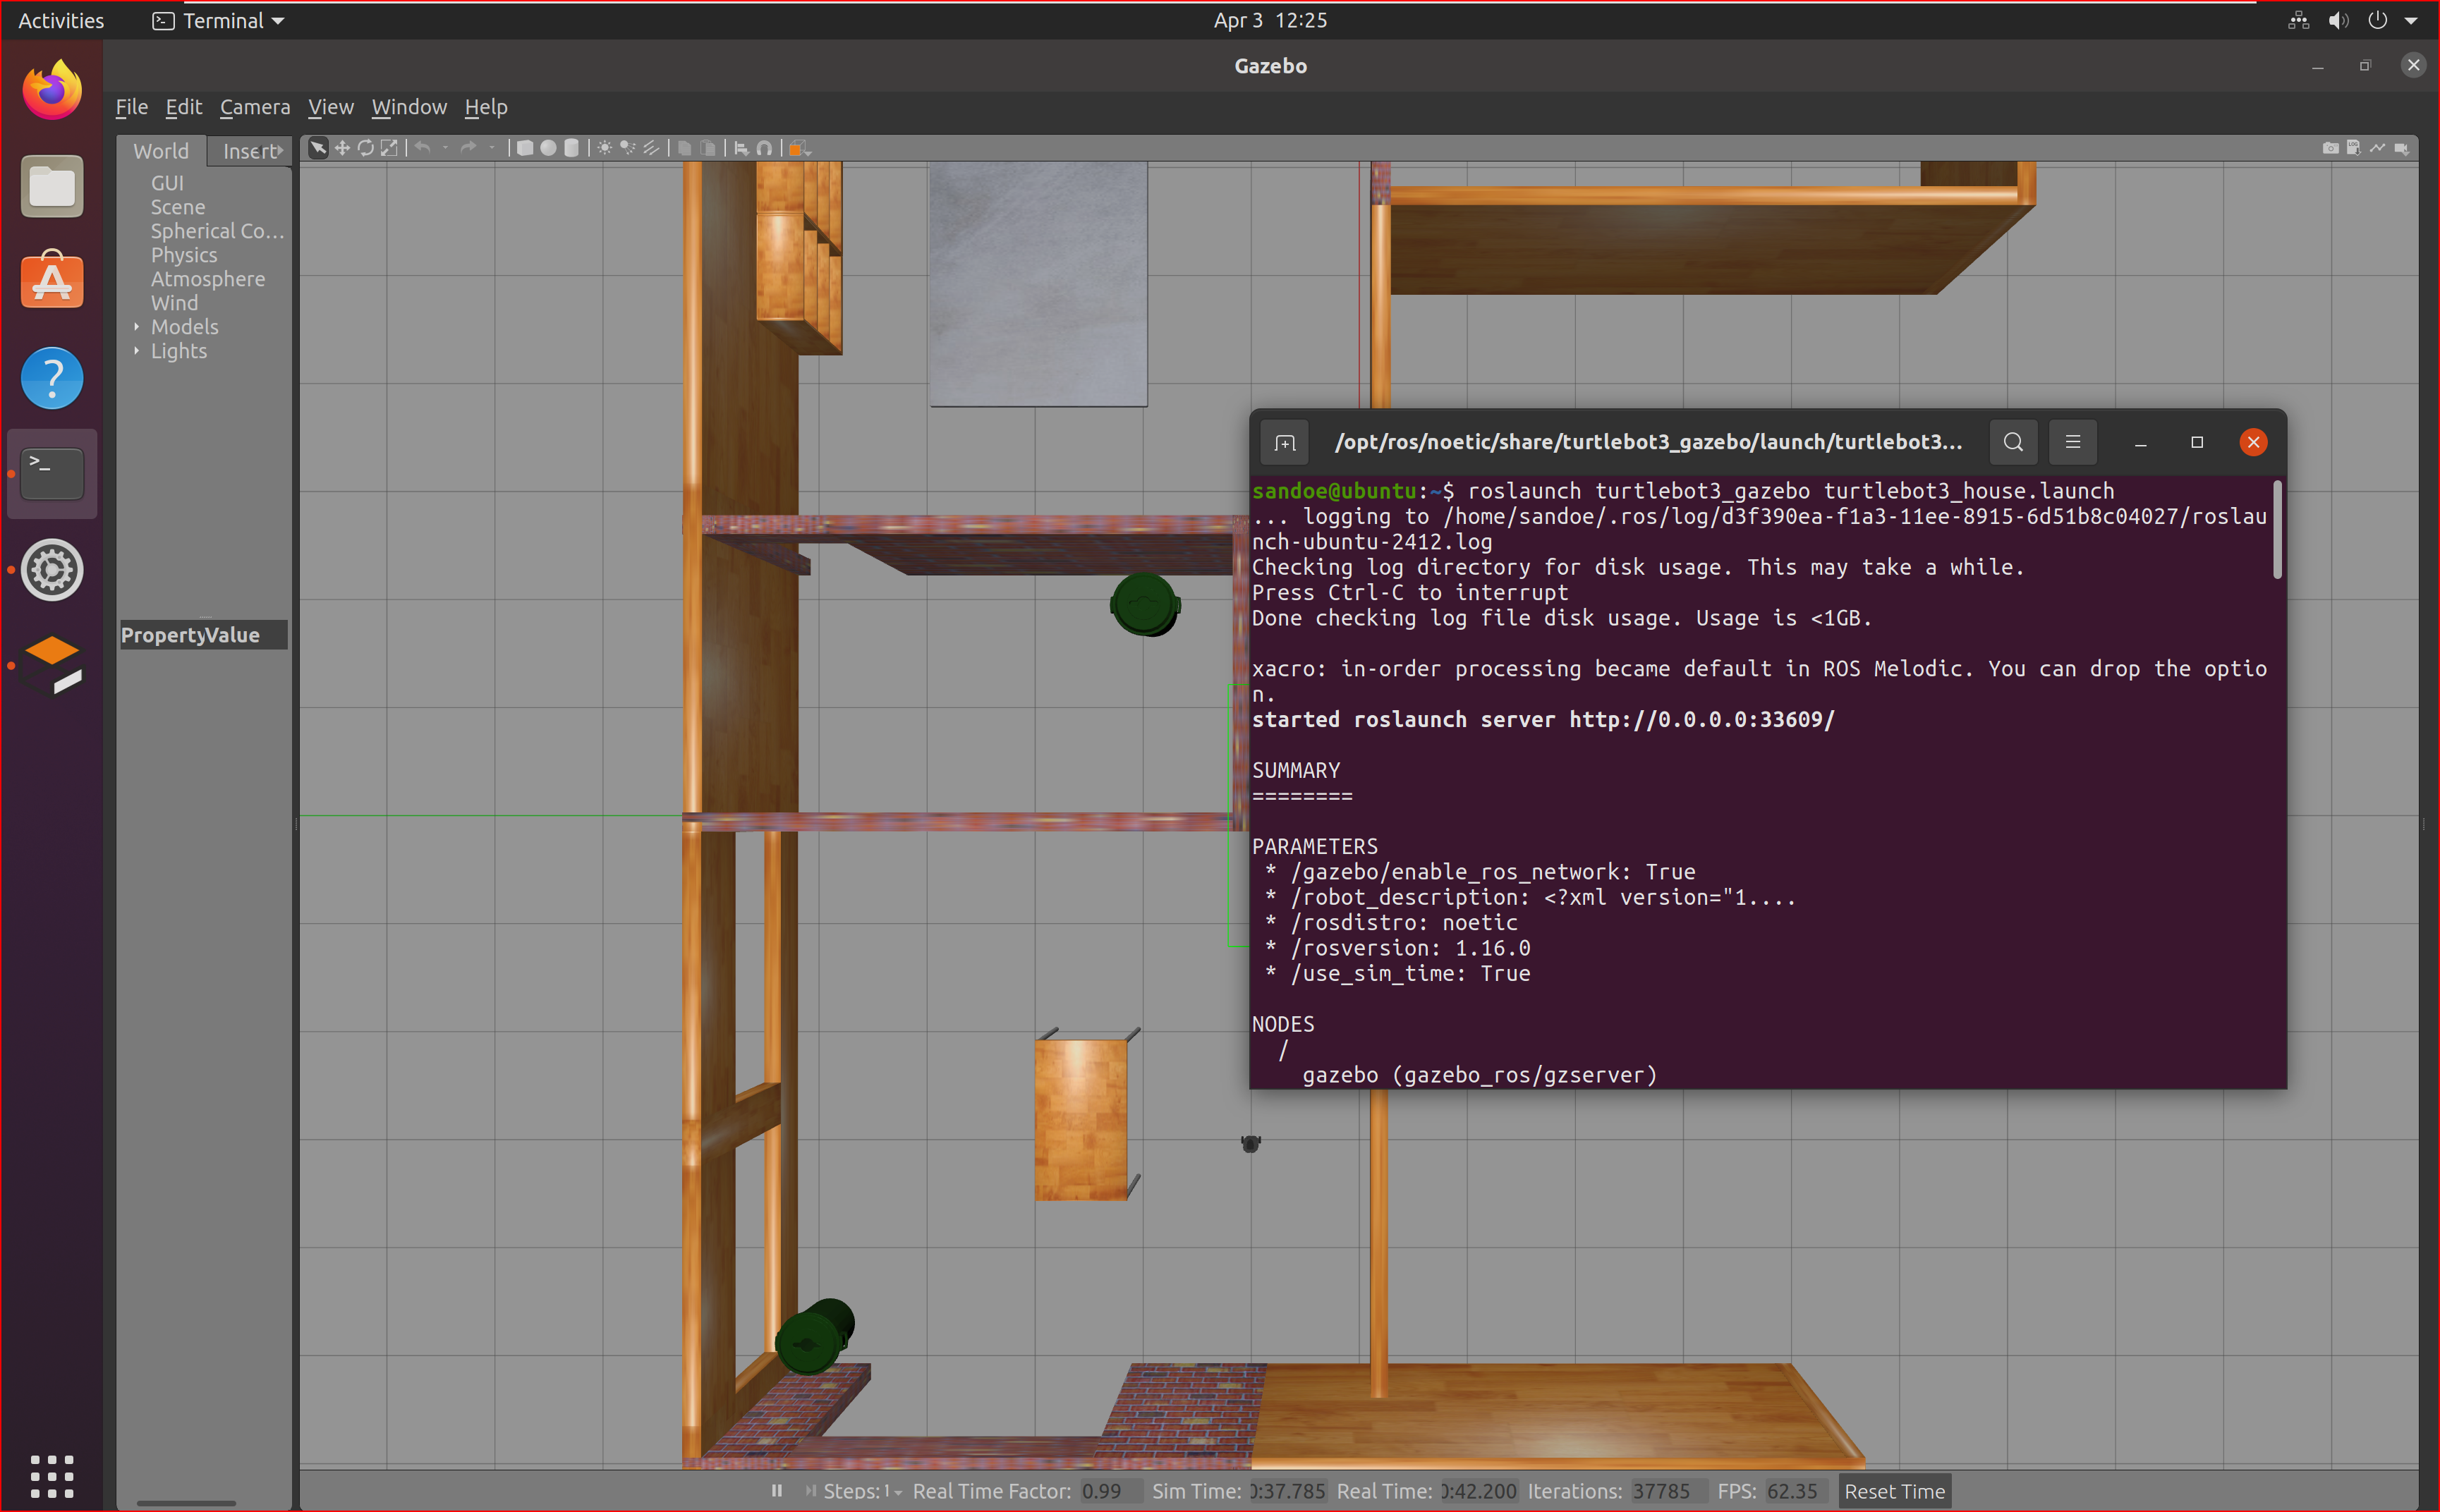
\includegraphics[width=\linewidth]{fig1.png}
		\caption{Simulation environment in Ubuntu (Fosscal), Gazebo V11 and Turtlebot3}
		\label{fig:fig1}
	\end{figure}
	
	\noindent The Turtlebot model is missing it's camera and therefore we need to terminate the session and navigate to the following folder \texttt{catkin\_ws} for then be using the command \texttt{source devel/setup.bash}. The purpose of this command it is to do the environment setting. We relaunch the simulation by following command:
	
	\noindent\texttt{roslaunch turtlebot3\_gazebo}\texttt{turtlebot3\_house.launch}.
	\\\\
	To verify that the camera and Lidar sensor is working then we run \texttt{rostopic list} (showing the list of ROS-topics) followed up by \texttt{rostopic echo /scan} (topic for Lidar) and \texttt{rostopic echo /camera/image\_raw} (topic for camera). By looking at the data stream in figure \ref{fig:fig5} then we can verify that the configuration is done and our environment is running.
	\begin{figure}[!h]
		\centering
		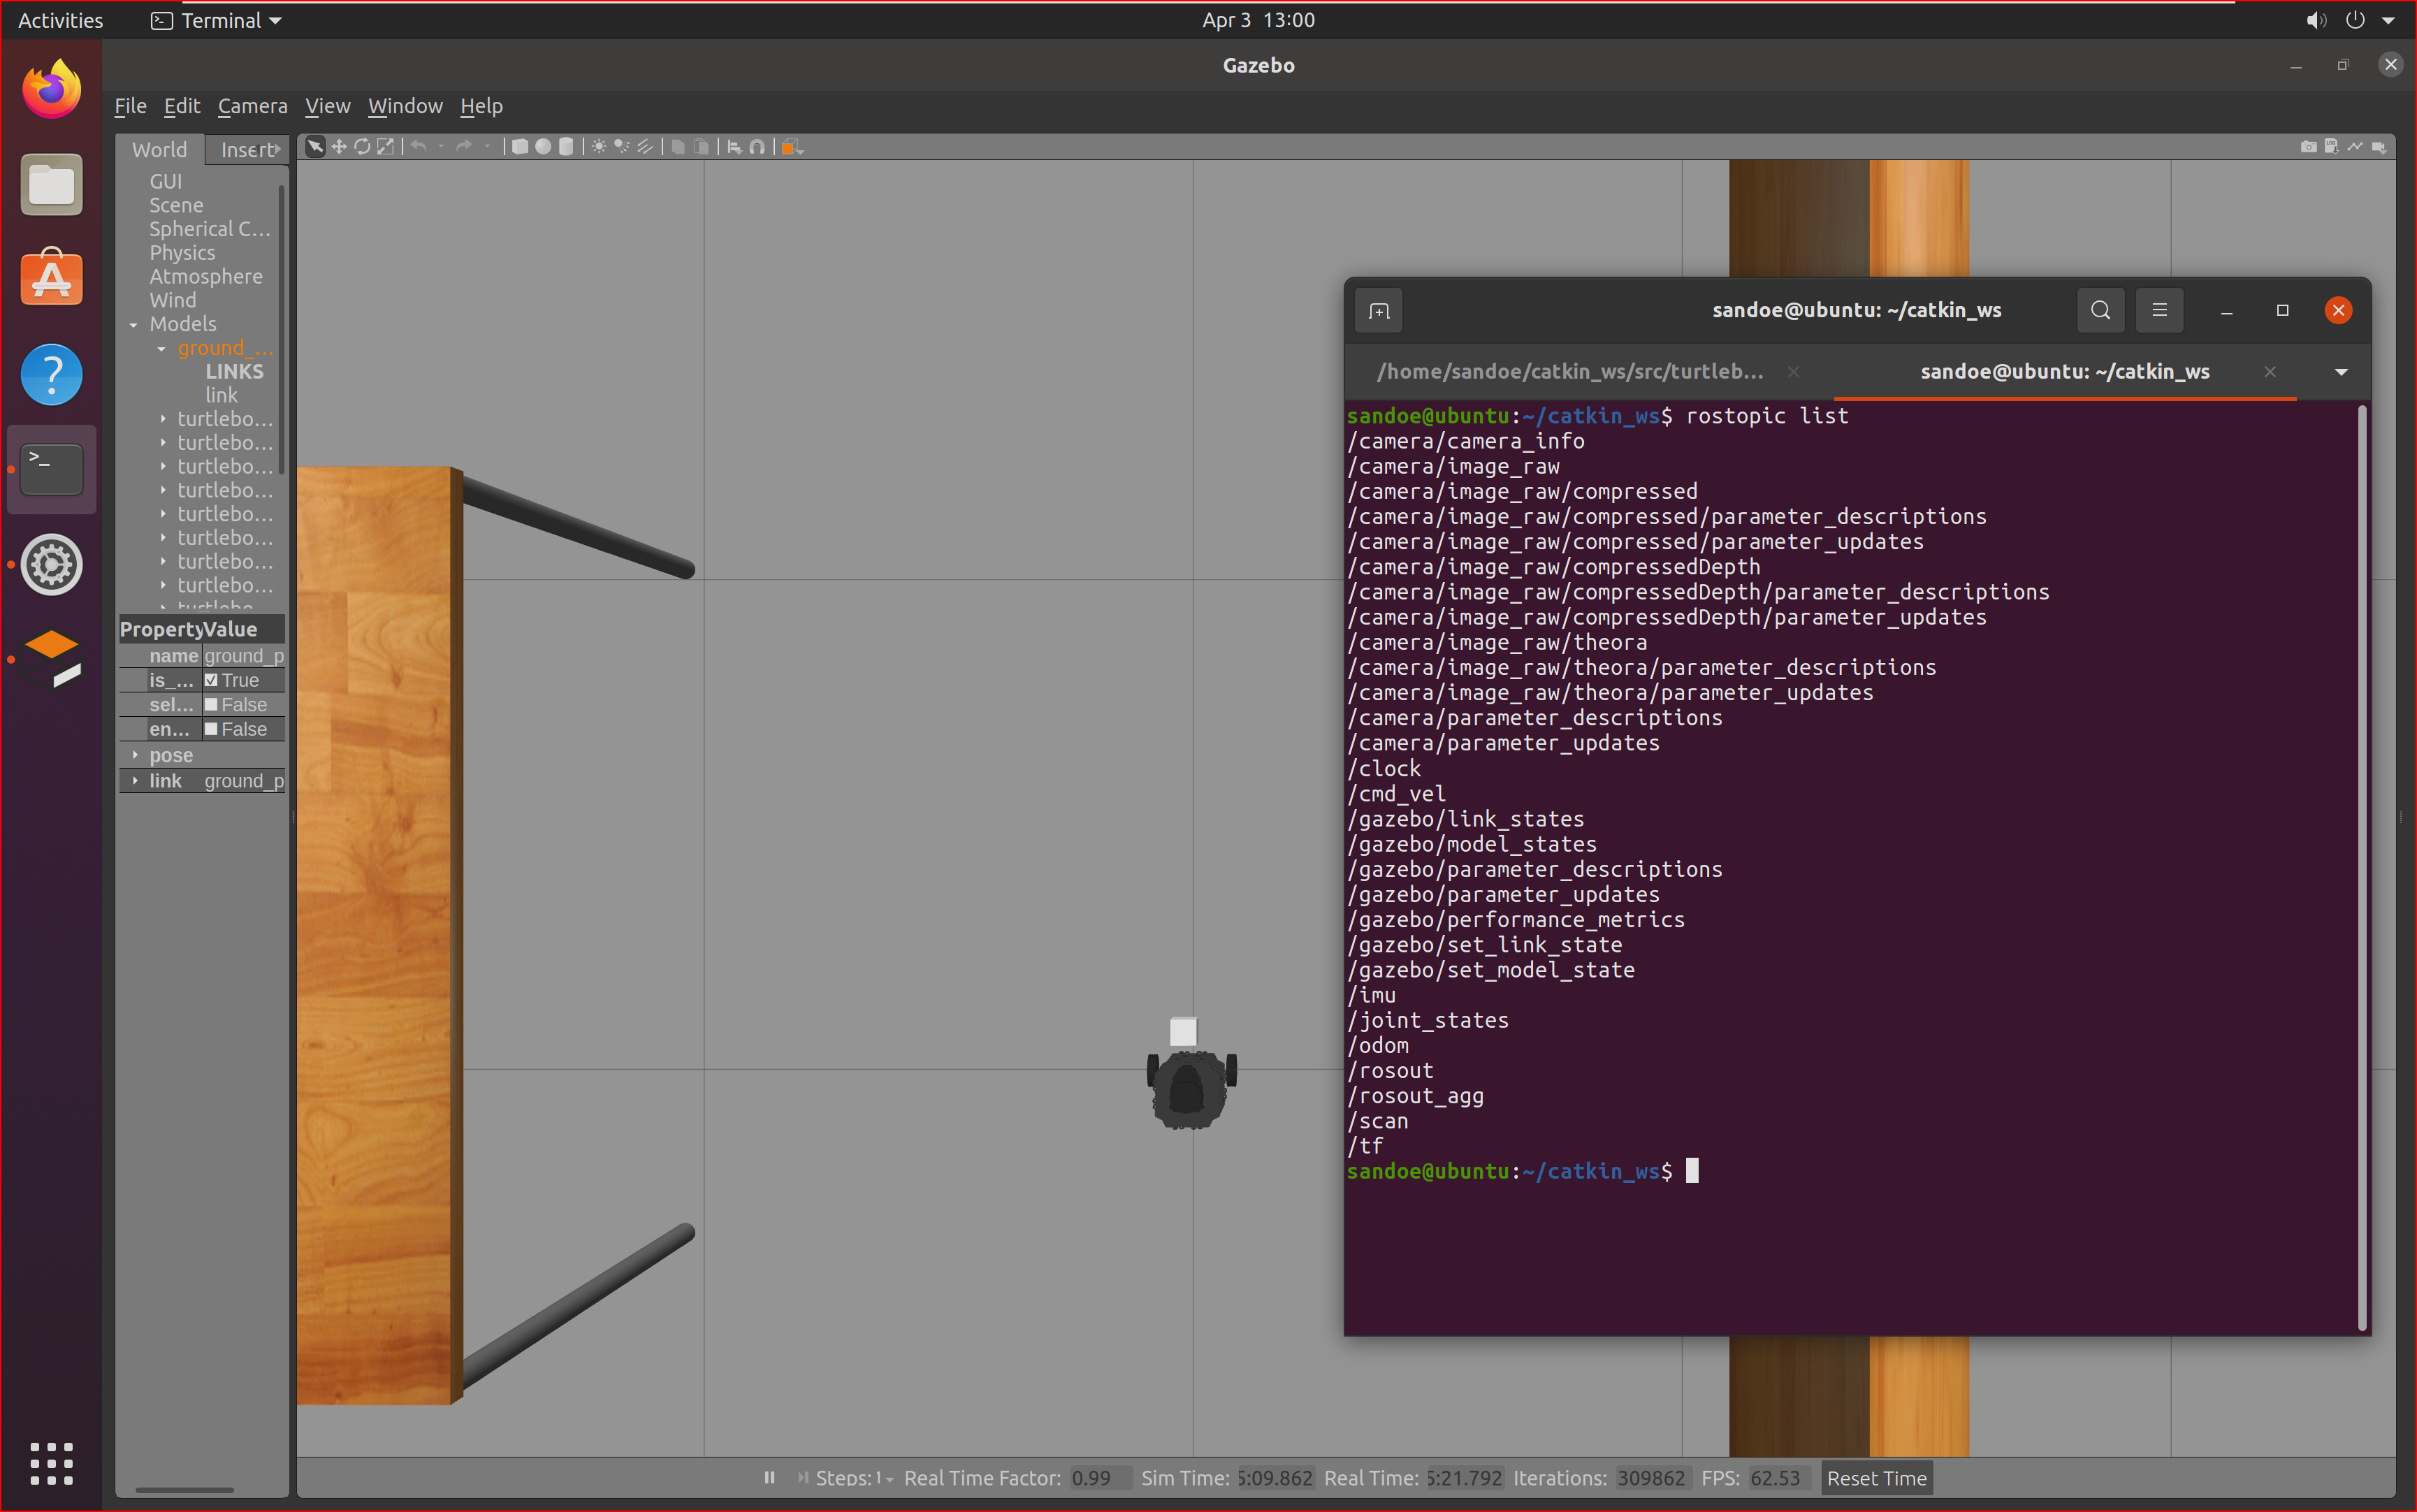
\includegraphics[width=\linewidth]{fig4.png}
		\caption{Showing rostopic list}
		\label{fig:fig4}
	\end{figure}
	\begin{figure}[!h]
		\centering
		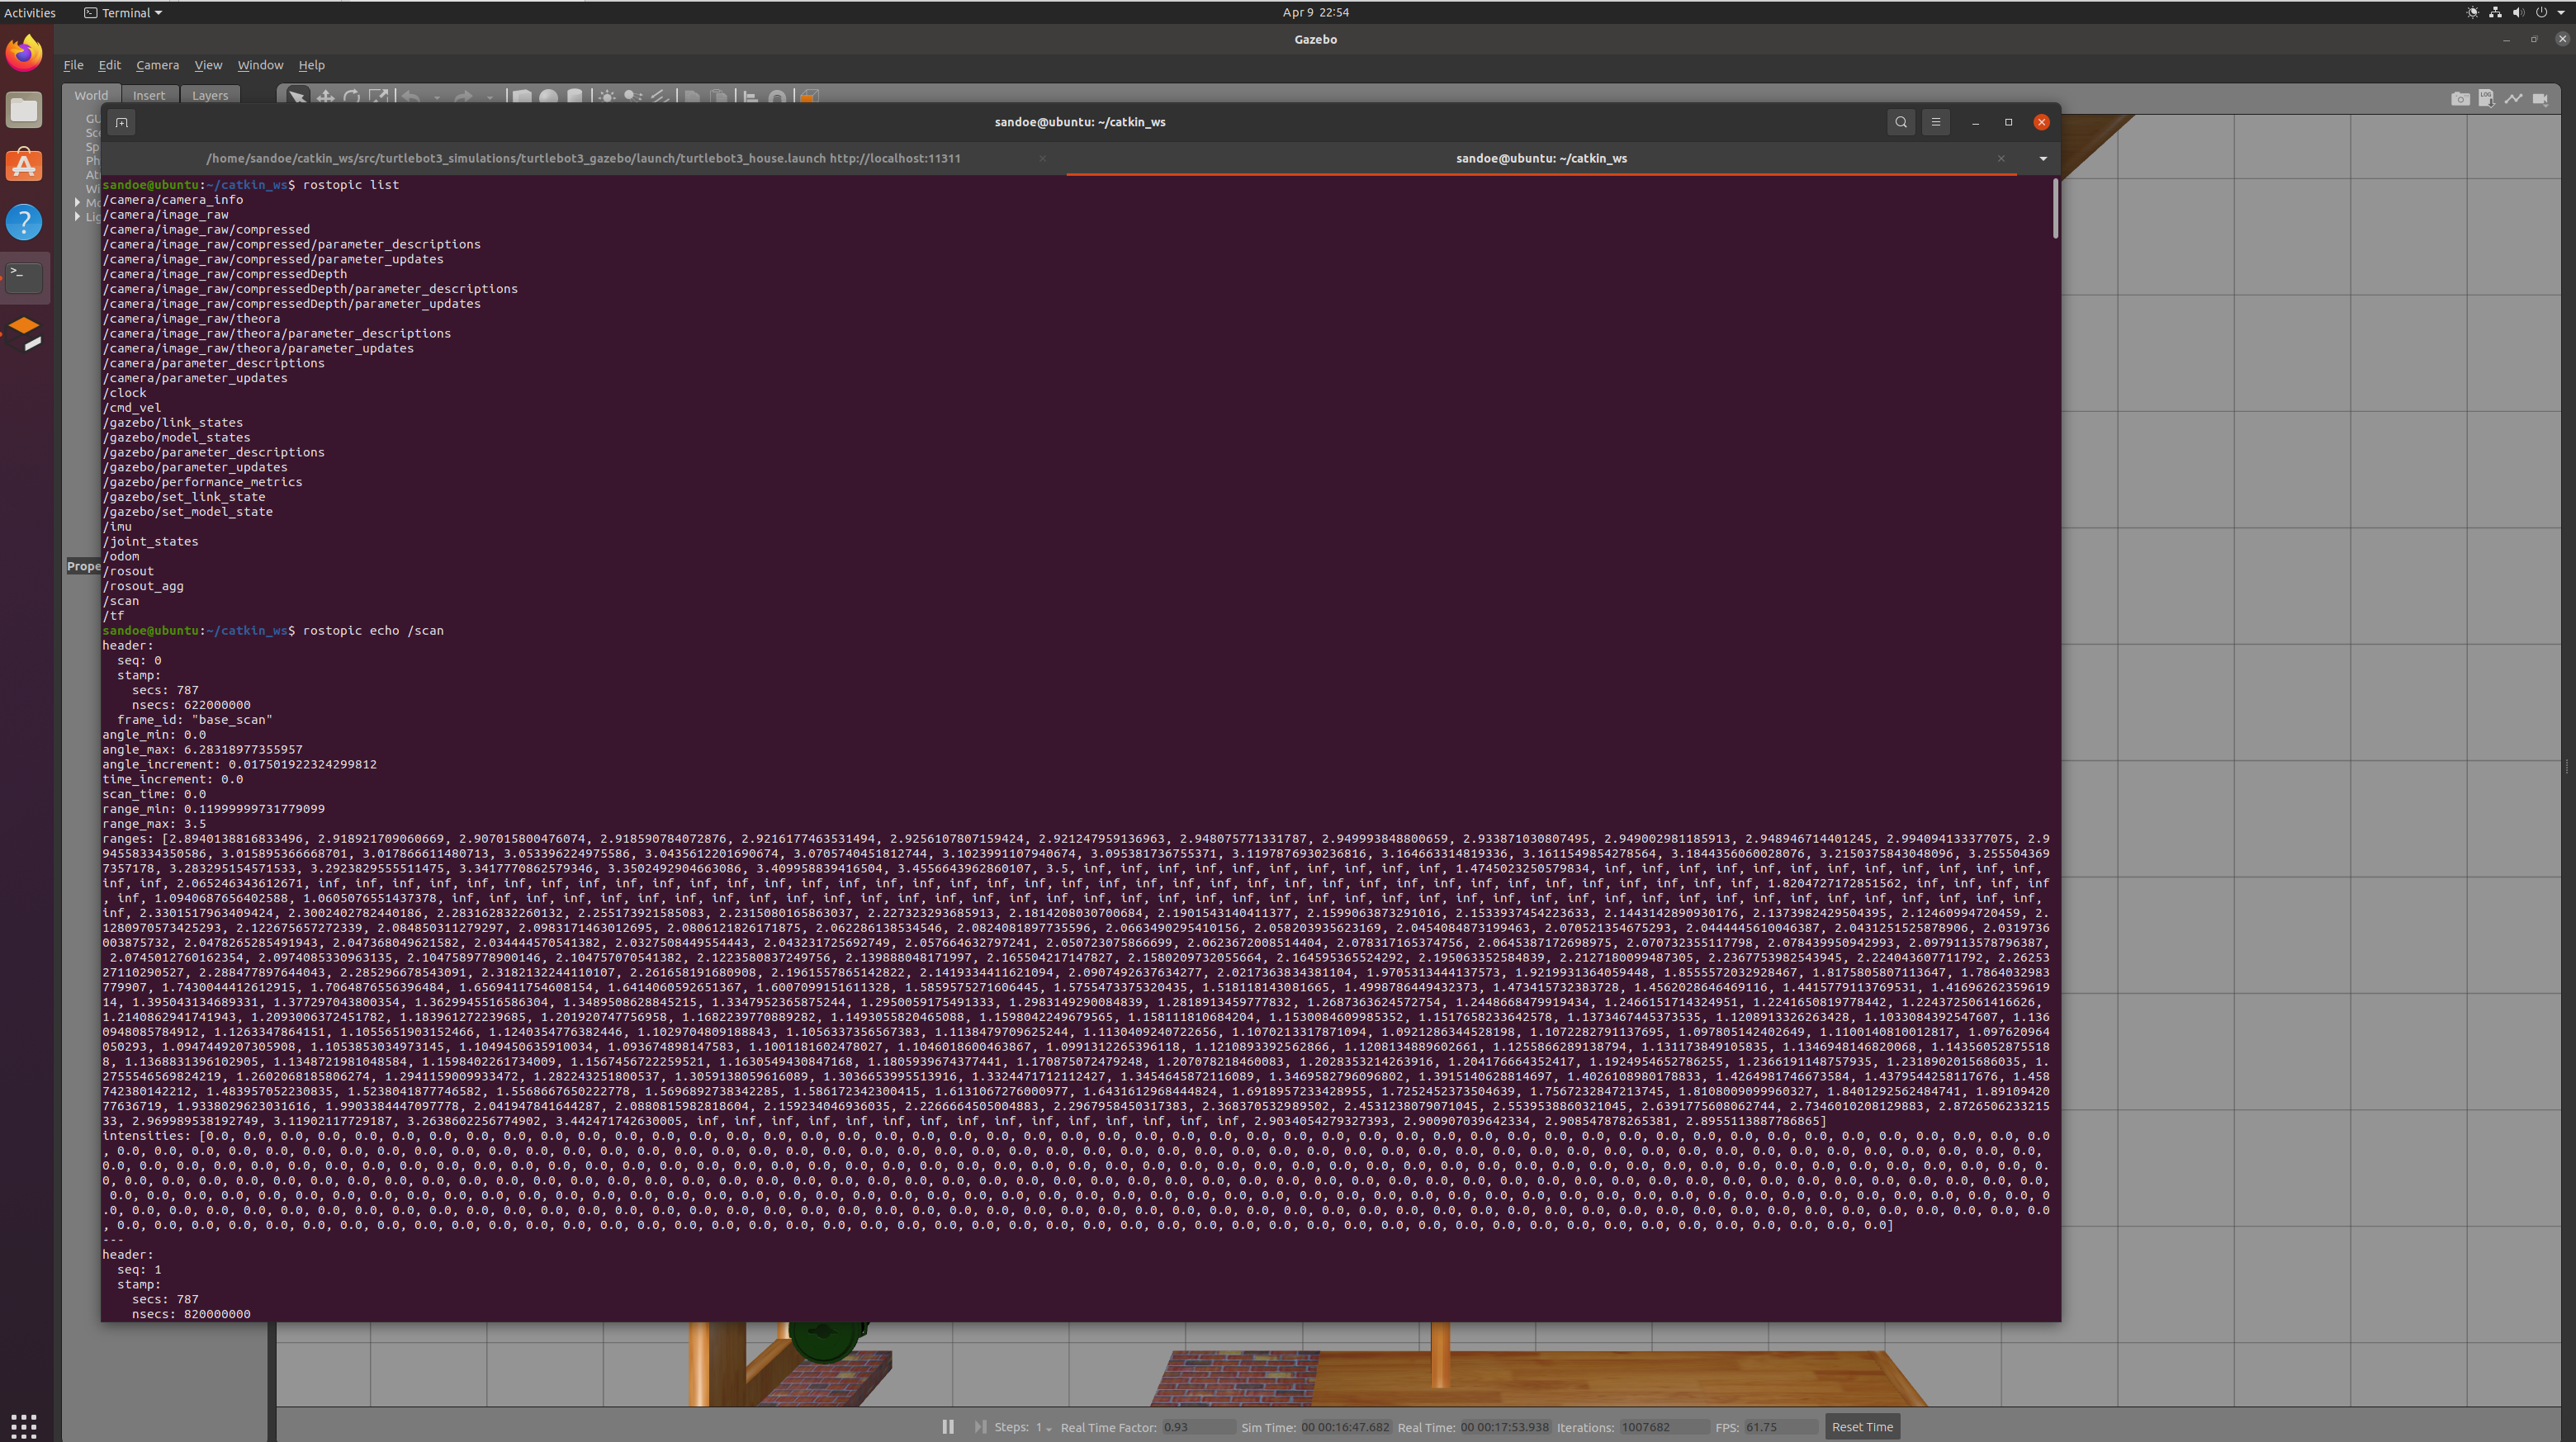
\includegraphics[width=\linewidth]{fig5.png}
		\caption{/scan data stream}
		\label{fig:fig5}
	\end{figure}
	\subsubsection{Matlab script}
	In this section there will be an introduction to the Matlab script for getting the values from the Lidar which is published on the topic \texttt{/scan}.
	\clearpage
	\begin{lstlisting}
	% Initialize ROS
	rosshutdown;
	rosinit('http://localhost:11311'); % Replace with your ROS master's URI
	
	%% Subscriber and publisher setup
	vel_pub = rospublisher('/cmd_vel');
	scansub = rossubscriber('/scan');
	pos_sub = rossubscriber('/tf');
	
	%% Controller setup
	controller = controllerPurePursuit;
	controller.DesiredLinearVelocity = 0.2;
	controller.MaxAngularVelocity = 2;
	
	%We found that the robot is relatively stable with a LookAheadDistance of
	%0.4
	controller.LookaheadDistance = 0.4;
	
	%Since we're using the reference frame of the LIDAR position and angle are
	%always 0
	robotCurrentPose = [0; 0; 0];
	
	while(1)
		%% Data retrieval
		scan = receive(scansub);
		cart = readCartesian(scan);
		
		hold on
		xlim([-4 4])
		ylim([-4 4])
		
		x = cart(:, 1);  % x-pos
		d = cart(:, 2);  % y-pos
		
		% Filter out points with y coordinates above 0 (to the right of the robot)
		filtered_indices = d <= 0;
		x = x(filtered_indices);
		d = d(filtered_indices);
		
		%% Fitting the line of the wall and plotting it
		
		mdl = fitlm(x,d);
		coef=mdl.Coefficients.Estimate;
		
		plot(x, (coef(1) + coef(2)*x), 'r')
		
		% Calculate the distance from the robot to the line to check if
		% distance is ~0.5 meter
		distance = abs(coef(1)) / sqrt(1 + coef(2)^2);
		
		fprintf('Closest distance from (0,0) to the line: %f\n', distance);
		
		%Defining a point to aim for 0.5 meters out from the wall and 1 meter
		%ahead
		aim_point = [1 0.5+(coef(2)*1+coef(1))];
		
		plot(aim_point(1),aim_point(2),'b.');
		
		%Setting the controller to go towards the aim-point
		controller.Waypoints = aim_point;
		[v, w] = controller(robotCurrentPose);
		update_vel(v,w,vel_pub)		
	end
	
	function [true] = update_vel(v,w,vel_pub)
		%Very simple function. We get a new linear and angular velocity from the
		%controller and output it to the cmd_vel topic.
		twistmsg = rosmessage(vel_pub);
		
		twistmsg.Angular.Z = w;
		twistmsg.Linear.X = v;
		
		send(vel_pub,twistmsg);
	end
	\end{lstlisting}
	A picture of the Turtlebot following the wall.
	\begin{figure}[!h]
		\centering
		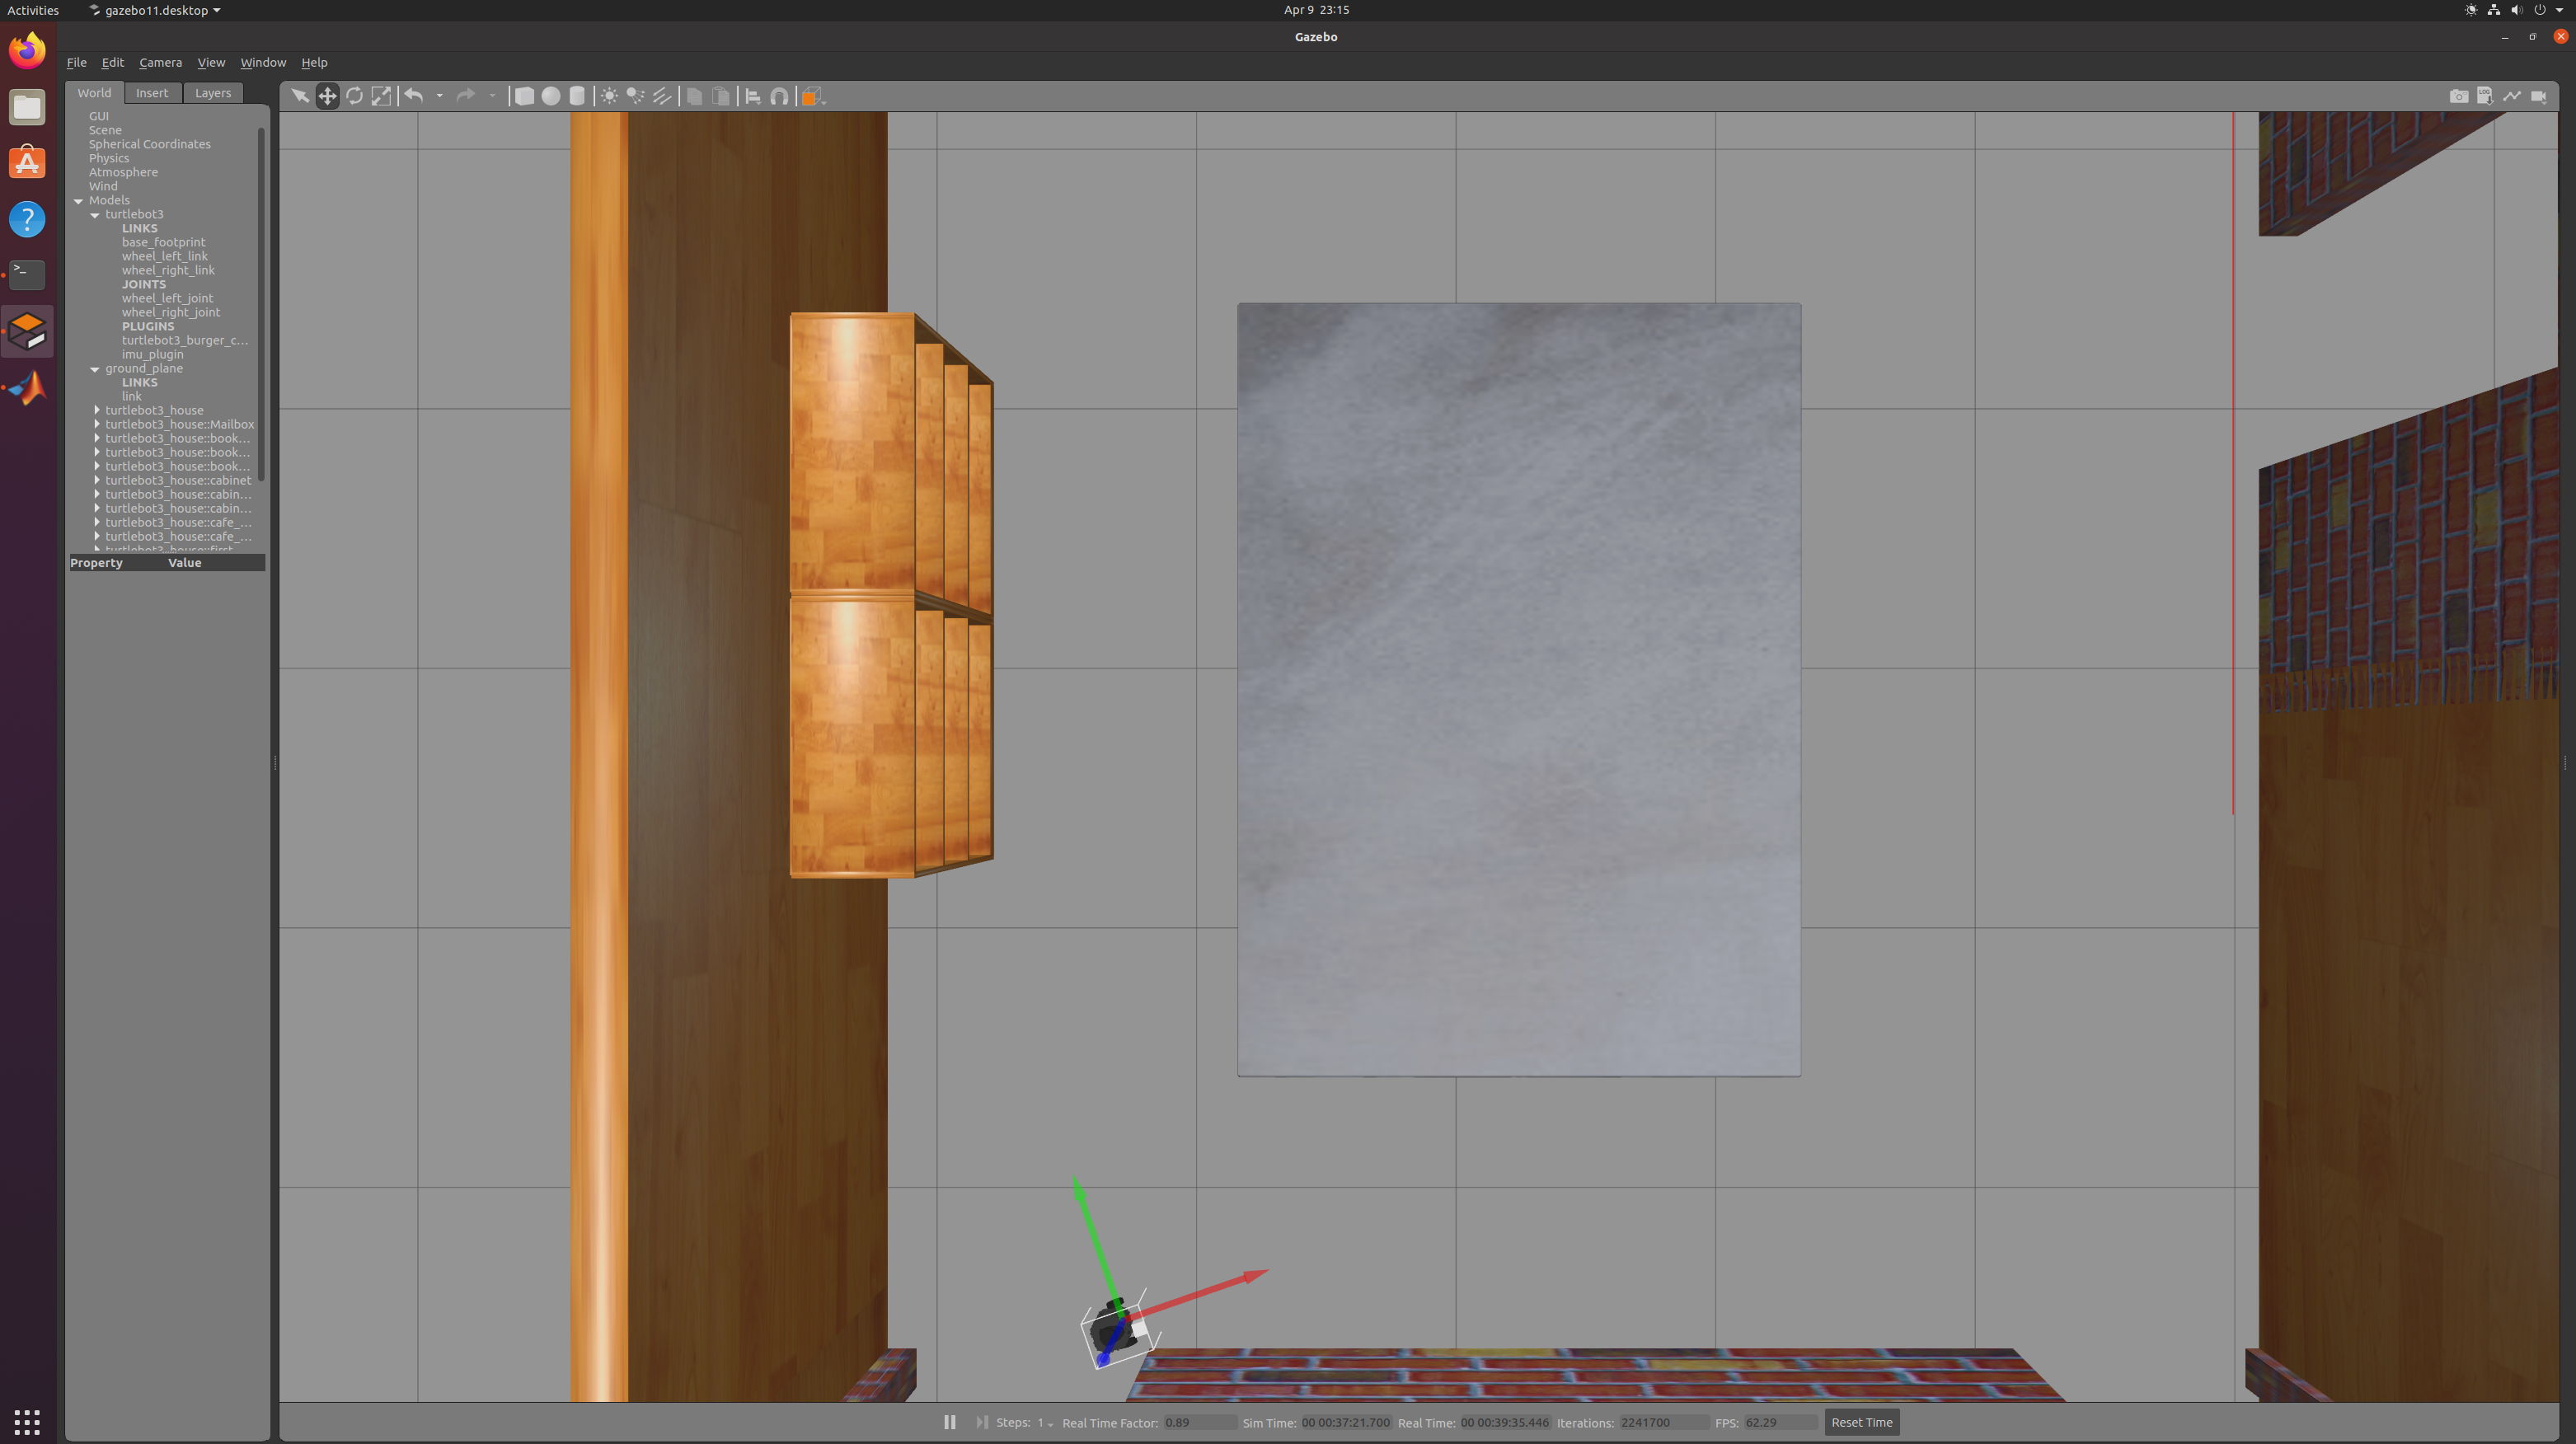
\includegraphics[width=\linewidth]{fig6.png}
		\caption{Turtlebot following the wall at the right side}
		\label{fig:fig6}
	\end{figure}
	\subsection{Physical TurtleBot Configuration}
	
	\noindent\textbf{Matlab script for whole program}
	\begin{lstlisting}
		setenv('ROS_MASTER_URI','http://192.168.179.100:11311');
		setenv('ROS_IP','192.168.179.38');
		rosshutdown()
		rosinit('http://192.168.179.100:11311','NodeHost','192.168.179.38')
		
		%% Subscriber and publisher setup
		vel_pub = rospublisher('/cmd_vel');
		scansub = rossubscriber('/scan');
		pos_sub = rossubscriber('/tf');
		
		%% Controller setup
		controller = controllerPurePursuit;
		controller.DesiredLinearVelocity = 0.2;
		controller.MaxAngularVelocity = 2;
		
		%We found that the robot is relatively stable with a LookAheadDistance of
		%0.4
		controller.LookaheadDistance = 0.4;
		
		%Since we're using the reference frame of the LIDAR position and angle are
		%always 0
		robotCurrentPose = [0; 0; 0];
		
		while(1)
			%% Data retrieval
			scan = receive(scansub);
			cart = readCartesian(scan);
			
			hold on
			xlim([-4 4])
			ylim([-4 4])
			
			x = cart(:, 1);  % x-pos
			d = cart(:, 2);  % y-pos
			
			% Filter out points with y coordinates above 0 (to the right of the robot)
			filtered_indices = d <= 0;
			x = x(filtered_indices);
			d = d(filtered_indices);
			
			%% Fitting the line of the wall and plotting it
			
			mdl = fitlm(x,d);
			coef=mdl.Coefficients.Estimate;
			
			plot(x, (coef(1) + coef(2)*x), 'r')
			
			% Calculate the distance from the robot to the line to check if
			% distance is ~0.5 meter
			distance = abs(coef(1)) / sqrt(1 + coef(2)^2);
			
			fprintf('Closest distance from (0,0) to the line: %f\n', distance);
			
			%Defining a point to aim for 0.5 meters out from the wall and 1 meter
			%ahead
			aim_point = [1 0.5+(coef(2)*1+coef(1))];
			
			plot(aim_point(1),aim_point(2),'b.');
			
			%Setting the controller to go towards the aim-point
			controller.Waypoints = aim_point;
			[v, w] = controller(robotCurrentPose);
			update_vel(v,w,vel_pub)		
		end
		
		function [true] = update_vel(v,w,vel_pub)
		
			%Very simple function. We get a new linear and angular velocity from the
			%controller and output it to the cmd_vel topic.
			twistmsg = rosmessage(vel_pub);
			
			twistmsg.Angular.Z = w;
			twistmsg.Linear.X = v;
			
			send(vel_pub,twistmsg);
		end
	\end{lstlisting}
	\paragraph{Results:}
	\begin{itemize}
		\item \textbf{Measure the distance to the wall using a measurement tape} — Ensure accuracy by taking multiple measurements at different points along the wall.
		\item \textbf{Make several measurements with the LIDAR sensor} — Repeat these measurements under similar conditions to ensure consistency.
		\item \textbf{Compare the tape measurements with the LIDAR data} — Analyze how closely the LIDAR measurements align with the manual measurements from the tape.
		\item \textbf{Try to identify if there are any random or systematic errors} — Look for patterns in discrepancies that might indicate consistent bias or irregular errors.
		\item \textbf{Use a best-fit line through all data points and actual measurements to the wall} — This statistical method will help you find the most accurate representation of the measured data, minimizing the overall error.
		\item \textbf{Use this value from the best fit as a reference point for the robot's orientation towards the wall} — Implement this calibrated value in your robot’s navigation algorithm to improve its accuracy when approaching or aligning with the wall. 
	\end{itemize}
	
	\paragraph{Error Differentiation:}
	In the discourse on errors, it is essential to differentiate between systematic and random errors. Systematic errors are consistent and directional biases that can be corrected through calibration. In contrast, random errors manifest as unpredictable fluctuations that calibration cannot eliminate. The random errors are inherent in any measurement and can be mitigated through statistical methods such as averaging over multiple observations.
	\clearpage
	\paragraph{Our process for calibration}
	We have chosen to implement the algorithm using a pure pursuit controller from the last exercise. To do this we constantly have to update the point that we’re aiming for. This is done in a few steps.
	\\\\
	The data is filtered so we only see the data on the side of the wall (in our case the right of the robot)
	A line is fitted to the data.
	We calculate a point that is 0.5m out from the wall 1 meter ahead of the robot.
	We set this point as the next waypoint and update the velocity to what is calculated by the pure pursuit controller.
	\\\\
	This way the robot constantly tries to stay 0.5m out from the wall. While the robot runs we have made a plot that shows what the robot is seeing:
	\begin{figure}[!h]
		\centering
		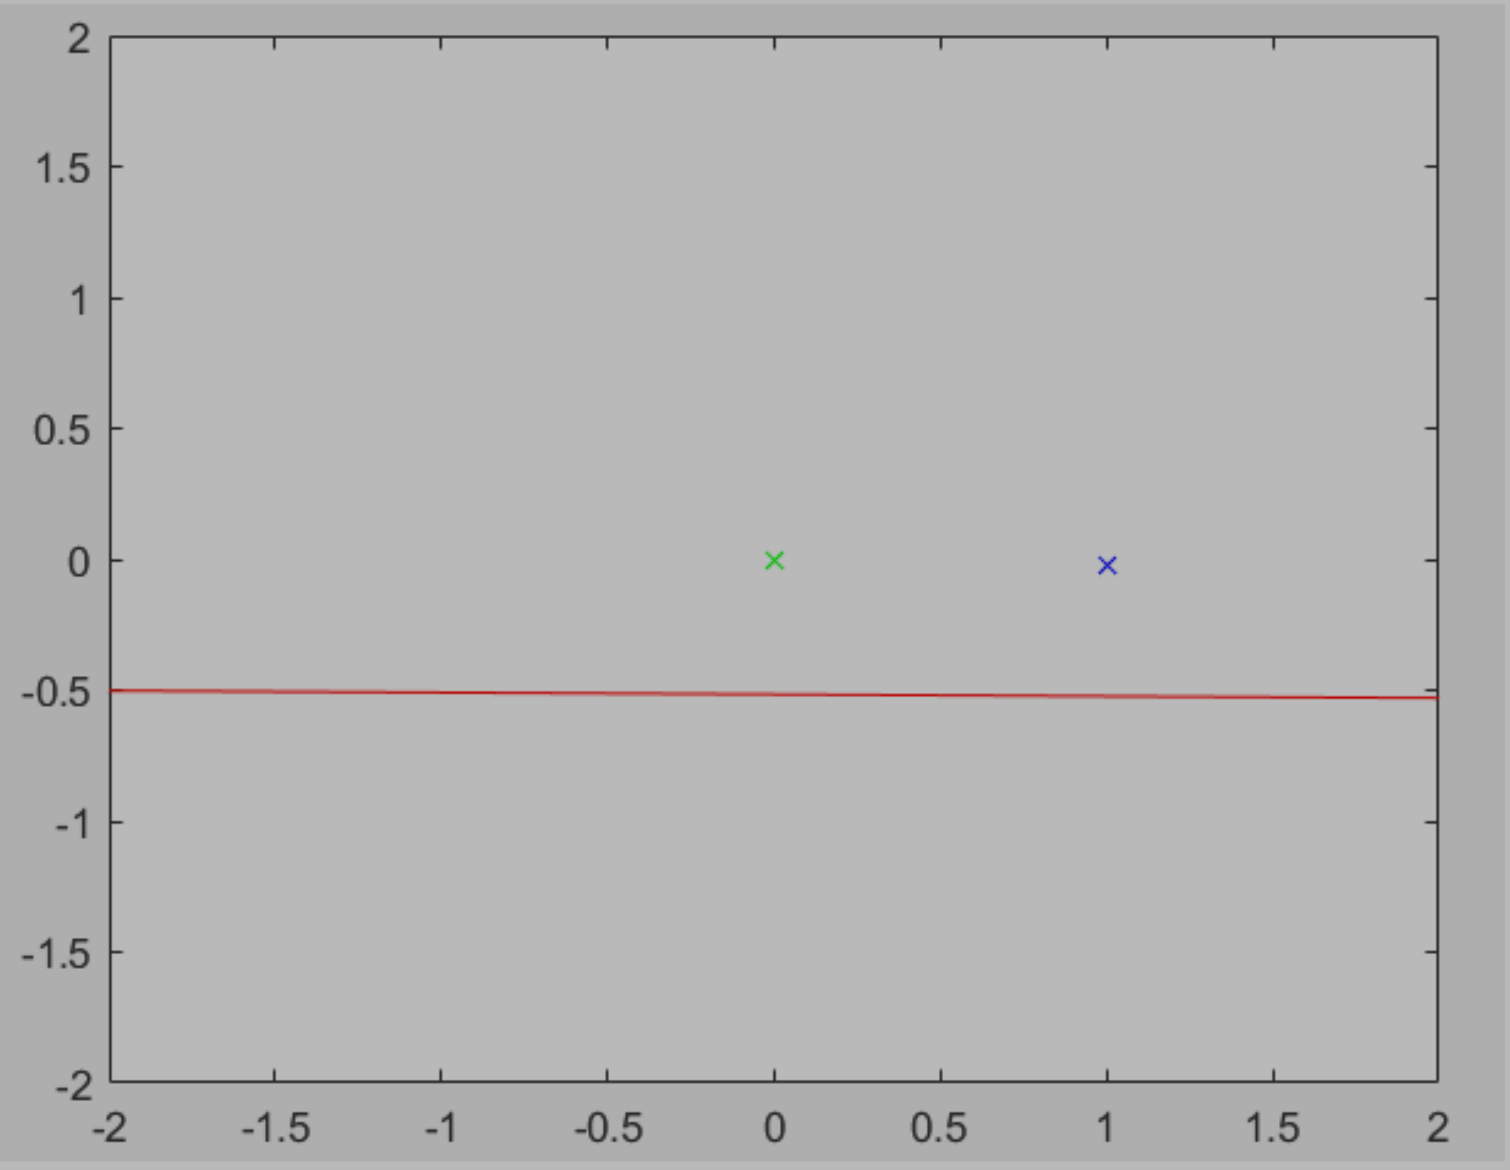
\includegraphics[width=\textwidth]{fig7}
		\caption{Showing green = robot, blue = waypoint, red = wall.}
		\label{fig:fig7}
	\end{figure}
	
	Here we can see that the wall is $\approx$0.5m from the robot and it has a point 1 meter out that it is aiming for. In the attached video you can also see a printout of how close the robot is to the red line aka. the approximation of the wall.
	\\\\
	When initializing the pure pursuit controller we have set the position of the robot to constantly be 0,0 and the orientation to be 0 degrees because we are driving from the LIDAR reference frame. 
\end{document}